\documentclass[border=1cm]{standalone}

\usepackage{tikz}

\begin{document}
    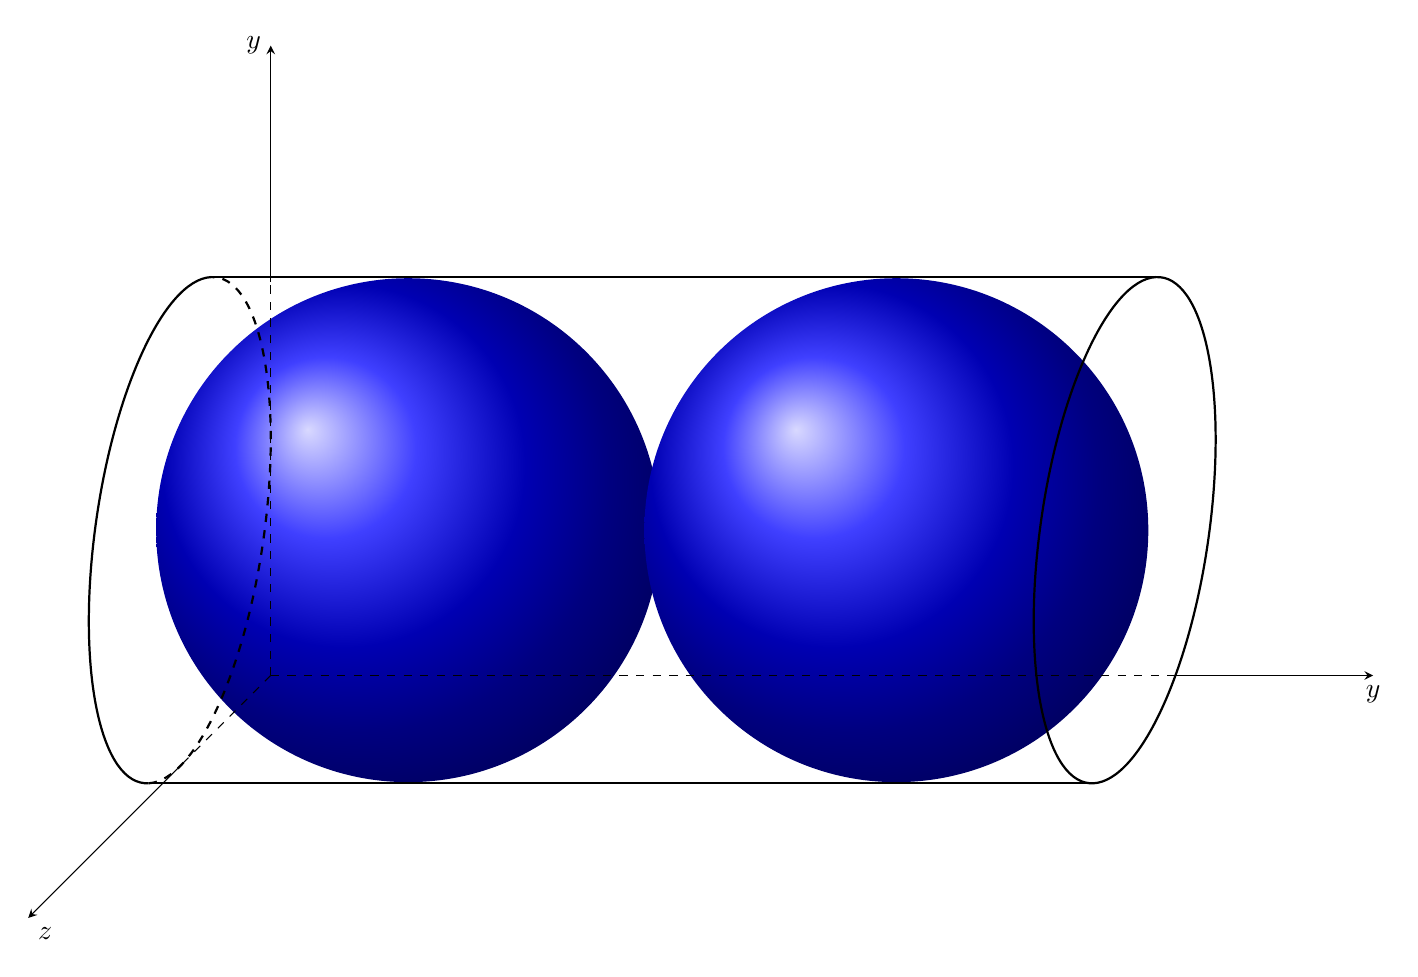
\begin{tikzpicture}
        \begin{scope}[thick, shift={(0,3,3)}, rotate around y=90, rotate around z=-20]
            \shade[ball color=blue] (0,0,2.9) circle (3.2 cm);
            \shade[ball color=blue] (0,0,9.1) circle (3.2 cm);
            \draw[dashed] (0,-3) arc [start angle=-90, end angle=90, radius=3];
            \draw (0,3) arc [start angle=90, end angle=270, radius=3];
            \draw (0,0,12) circle [radius=3];
            \draw (0,3)--(0,3,12) (0,-3)--(0,-3,12);
        \end{scope}
        \draw[dashed] (0,0)--(11.5,0);
        \draw[->,>=stealth] (11.5,0)--(14,0) node[below]{$y$};
        \draw[dashed] (0,0)--(0,5);
        \draw[->,>=stealth] (0,5)--(0,8) node[left]{$y$};
        \draw[dashed] (0,0,0)--(0,0,3);
        \draw[->,>=stealth] (0,0,3)--(0,0,8) node[below right]{$z$};
    \end{tikzpicture}
\end{document}